\documentclass{article}%
\usepackage[T1]{fontenc}%
\usepackage[utf8]{inputenc}%
\usepackage{lmodern}%
\usepackage{textcomp}%
\usepackage{lastpage}%
\usepackage{graphicx}%
%
\title{R) {[}1,2{]}\_ To date,three isotypes of PPARs, a, b, and c, have}%
\author{\textit{Kuo Lee}}%
\date{02-06-2009}%
%
\begin{document}%
\normalsize%
\maketitle%
\section{I am confident that the high{-}profile case of Cuban democrat Juan Agudelo, who was arrested and charged with an offence relating to the 2008 Cuban coup, has given Jamaica its advance perception of the region}%
\label{sec:Iamconfidentthatthehigh{-}profilecaseofCubandemocratJuanAgudelo,whowasarrestedandchargedwithanoffencerelatingtothe2008Cubancoup,hasgivenJamaicaitsadvanceperceptionoftheregion}%
I am confident that the high{-}profile case of Cuban democrat Juan Agudelo, who was arrested and charged with an offence relating to the 2008 Cuban coup, has given Jamaica its advance perception of the region.\newline%
Let us not forget, that Agudelo took into consideration the recent divergence of moods between India and Cuba at the G8 Summit {-}a move labelled as a major breakthrough. Ajit Amrith, lecturer at UWI and a political scientist, concurred, that Cuba is being watched as an opportunity for decades to come.\newline%
However, Guyanese have been less impressed with Agudelo's case. Interestingly, Ajiv Din, Professor of Law at UNSW, who submitted a rebuttal document to the Government proposing as a reason why Agudelo should not be punished with the threat of death under Rule 505 of the Criminal Code, has voiced concern that Agudelo's arrest stems from the pronouncement by several prominent intellectuals such as Dr Sasdev{-}Ram, Phillip D. Giroux, Warren Q. Richardson, Steven T. Hall, C.M., Zoéon Hornus and William T. David, and like others it seems that Agudelo is telling a story of a peaceful revolutionary revolution in which he joined forces with a number of well{-}trained political revolutionaries to overthrow the Cuban regime.\newline%
Does anyone doubt that Agudelo does still have a long way to go before he is fully exonerated by law? It is vital that he is released soon. Until we are properly investigated and, according to the Jamaica Constabulary Force, killed by the Fulcrum regime, the case will continue.\newline%

%


\begin{figure}[h!]%
\centering%
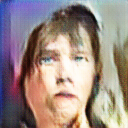
\includegraphics[width=120px]{./photos_from_epoch_8/samples_8_284.png}%
\caption{a man in a suit and tie holding a tennis racket .}%
\end{figure}

%
\end{document}